\documentclass[12pt]{ai_conquer2026}
\addbibresource{references.bib}

\title{%
  \begin{center}
        \Large {AI VIET NAM -- AI Conquer 2026}\\[.5ex]
        \Huge \textbf{Player Style Clustering from Football Event Data:\\[.3ex]
        A K-Means Study on Scaling, Model Selection, and Stability}\\[.5ex]
  \end{center}
}

% Author --------------------------------------------------------------------
\posttitle{
\author{
\begin{minipage}{\textwidth}
\centering
{
\vspace{-1.5em}
Group: Nguyễn Thanh Phong (Team Lead) $\cdot$ Võ Công Tuấn Lộc (Data Engineer) $\cdot$ Trương Hoàng Thông (ML \& Eval Engineer)
}\\
\end{minipage}
}
}
\date{}

% Header --------------------------------------------------------------------
\pagestyle{fancy}
\fancyhf{}
\lhead{\href{https://www.facebook.com/aivietnam.edu.vn}{\textcolor{aivnGreen}{\bfseries AI VIET NAM (AI Conquer 2026)}}}
\rhead{\href{https://aivietnam.edu.vn/}{\textcolor{aivnGreen}{\bfseries aivietnam.edu.vn}}}
\fancyfoot[C]{\thepage}
\renewcommand{\headrulewidth}{1.0pt}
\renewcommand{\headrule}{{\color{aivnGreen}\hrule width\headwidth height\headrulewidth \vskip-\headrulewidth}}

\begin{document}

% Override Vietnamese labels from .cls for English report
\renewcommand{\contentsname}{Table of Contents}
\renewcommand{\refname}{References}
\renewcommand{\figurename}{Figure}
\renewcommand{\tablename}{Table}
\renewcommand{\capfig}[1]{%
  \refstepcounter{hinh}%
    Figure~\thehinh:~#1
}
\renewcommand{\appendixtocname}{Appendices}
\renewcommand{\appendixpagename}{Appendices}

\maketitle
\vspace{-5.5em}

% --------------------------------------------------------------------------
\section{Abstract}

Clustering player styles is an important topic in modern football analytics, with practical applications in tactical profiling, opposition analysis, and player recruitment. Although K-Means is a standard clustering method, its performance depends strongly on feature scaling, the choice of the number of clusters $k$, and proper validation. In football event data, metrics often have skewed distributions due to standout players (such as top goalscorers and high-volume playmakers), making traditional normalization methods sensitive to distortion.

In this study, we present a practical approach to unsupervised player style clustering using K-Means. We analyze 1,016 qualified players ($\ge 900$ minutes played) across 1,140 matches from the 2015/2016 season in three major European leagues (Premier League, La Liga, and Serie A) using open StatsBomb event data. Each player is represented by 29 per-90 rate and efficiency metrics covering shooting, passing, dribbling, defense, and pitch coordinates.

Our main findings are:
\begin{enumerate}
    \item \textbf{Robust Scaling is Essential:} Using median and interquartile range normalization (RobustScaler) effectively handles extreme values, clearly outperforming raw unscaled features and standard z-score normalization.
    \item \textbf{Optimal Number of Clusters ($k=5$):} Although the Silhouette score peaks at $k=2$ (a simple split into defensive and offensive players), choosing $k=5$ provides the best balance between statistical quality and meaningful tactical roles.
    \item \textbf{High Stability and Clear Boundaries:} The five clusters align well with real playing positions (purity $\approx 69.7\%$, $\text{NMI} \approx 0.546$). Furthermore, a supervised K-Nearest Neighbors (KNN) classifier achieves $96.6\% \pm 0.8\%$ 5-fold cross-validation accuracy, showing that the clusters have well-defined decision boundaries.
    \item \textbf{Striker Sub-Clustering (Case Study):} A secondary clustering step on the 152 strikers reveals three distinct tactical roles: Poachers, Target Men, and Deep-Lying Forwards. This shows that the pipeline can be extended hierarchically to discover more specific player styles.
\end{enumerate}

\newpage
\setcounter{tocdepth}{2}
\tableofcontents
\thispagestyle{fancy}

% --------------------------------------------------------------------------
\newpage
\section{Introduction}

In recent years, data analytics has reshaped how football clubs and scouts assess player performance. In the past, player evaluation relied heavily on visual scouting and basic statistics such as total goals, assists, or clean sheets. However, modern football features fluid tactics, pressing systems, and flexible roles (such as inverted fullbacks, false nines, and roaming playmakers). As a result, broad positional labels (e.g., "Midfielder" or "Defender") often fail to capture the actual roles that players perform on the pitch over a full season.

With the availability of detailed event data from providers like StatsBomb \cite{statsbomb_open_data}, every action on the ball—including passes, shots, pressures, recoveries, and spatial locations—is recorded accurately. This granular information allows analysts to build behavioral profiles that reflect what players actually do during matches. Unsupervised machine learning, particularly clustering, provides a structured way to discover natural player archetypes directly from these event distributions.

However, applying K-Means clustering \cite{macqueen1967methods} to football data involves several practical challenges:
\begin{itemize}
  \item \textbf{Scale Differences and Skewed Data:} Event metrics differ greatly in scale. For instance, a central midfielder may attempt over 60 passes per match, whereas a striker may take only 2 or 3 shots. In addition, outstanding individual performances create heavily skewed distributions. Without suitable scaling, standard distance metrics such as Euclidean distance become dominated by high-volume features.
  \item \textbf{Choosing the Number of Clusters ($k$):} Determining the best value of $k$ requires balancing mathematical criteria against practical interpretability. Pure statistical metrics often favor simple two-cluster splits (such as dividing players into defenders and attackers), which are too broad for tactical analysis.
  \item \textbf{Cluster Validation and Stability:} Unsupervised clusters can easily be affected by random initialization. It is therefore essential to validate the results against real-world domain benchmarks and test their boundary stability.
\end{itemize}

This study addresses these challenges through a systematic analysis using full 2015/2016 season data from three major European leagues. Importantly, ground-truth player positions (\texttt{primary\_position}) are kept strictly as hidden evaluation labels and are never used during feature engineering or cluster fitting.

\textbf{Research Questions:}
\begin{itemize}
  \item \textbf{RQ1 (Feature Scaling Impact):} How do different scaling methods (Unscaled, StandardScaler, RobustScaler) affect feature distributions and the resulting K-Means clusters?
  \item \textbf{RQ2 (Optimal Cluster Resolution):} Which number of clusters $k \in [2, 10]$ provides the best balance across the Elbow method (WCSS), Silhouette Score, and Gap Statistic?
  \item \textbf{RQ3 (Tactical Alignment and Stability):} How well do the unsupervised clusters match real-world playing positions, and how stable are the cluster boundaries under supervised classification?
\end{itemize}

\textbf{Paper Organization:} The rest of this paper is organized as follows: Section~\ref{sec:related_work} reviews related literature on football analytics and clustering methods. Section~\ref{sec:methodology} presents the mathematical foundations of K-Means, scaling techniques, and evaluation metrics. Section~\ref{sec:data} describes data collection, player filtering, and feature extraction. Section~\ref{sec:results} presents the main experimental results, model selection curves, tactical interpretations, and stability tests. Section~\ref{sec:discussion} discusses practical applications for scouting and recruitment, and Section~\ref{sec:conclusion} concludes the paper.

% --------------------------------------------------------------------------
\section{Related Work}
\label{sec:related_work}

Player profiling and tactical clustering in football have developed across three main areas:

\subsection{Positional vs. Behavioral Profiling}
Traditional sports analysis categorized players mainly by their nominal starting positions on team sheets. However, modern tactical systems require players to carry out multiple functions regardless of their listed position. Recent sports analytics research focuses on behavioral profiling derived from match events and tracking coordinates \cite{pedregosa2011scikit}. By aggregating event counts into per-90 rates and spatial metrics, analysts can identify functional player roles and tactical versatility without being constrained by fixed positional categories.

\subsection{Distance-Based Clustering in Sports}
The K-Means algorithm \cite{macqueen1967methods} remains widely used in sports analytics because of its computational efficiency and straightforward centroid-based cluster representations. However, distance-based algorithms that use Euclidean geometry are sensitive to feature scales and outliers. Standard normalization methods, such as $z$-score standardization, use the mean and standard deviation, which can be distorted by extreme performances \cite{hubert1985comparing}. While robust scaling based on medians and interquartile ranges is well established in statistics, direct comparisons of scaling resilience on multi-league football data remain relatively rare.

\subsection{Cluster Validation and Stability}
A common challenge in applied unsupervised learning is the need for reliable validation. Clustering algorithms will partition any dataset into $k$ groups, even when no natural groupings exist. Thorough validation requires two perspectives: (1) internal validation metrics, such as the Silhouette index \cite{rousseeuw1987silhouettes} and the Gap Statistic \cite{tibshirani2001estimating}, which measure cluster cohesion and separation against reference distributions; and (2) external validation and stability testing, where cluster labels are compared against domain positions and verified for boundary learnability using supervised classifiers such as K-Nearest Neighbors (KNN).

% --------------------------------------------------------------------------
\section{Methodology}
\label{sec:methodology}

This section describes the mathematical formulation of K-Means, the normalization methods, and the evaluation metrics used in this study.

\subsection{K-Means Formulation}
Let $X = \{\mathbf{x}_1, \mathbf{x}_2, \ldots, \mathbf{x}_n\} \subset \mathbb{R}^d$ represent the dataset of $n = 1016$ players, where each player vector $\mathbf{x}_i \in \mathbb{R}^{29}$ consists of 29 normalized performance features. The goal of K-Means is to partition the $n$ observations into $k$ disjoint clusters $C = \{C_1, C_2, \ldots, C_k\}$ to minimize the Within-Cluster Sum of Squares (WCSS):

\begin{equation}
\text{WCSS}(C) = \sum_{j=1}^{k} \sum_{\mathbf{x}_i \in C_j} \|\mathbf{x}_i - \boldsymbol{\mu}_j\|^2
\end{equation}

where $\boldsymbol{\mu}_j$ is the centroid representing the arithmetic mean of cluster $C_j$:

\begin{equation}
\boldsymbol{\mu}_j = \frac{1}{|C_j|} \sum_{\mathbf{x}_i \in C_j} \mathbf{x}_i
\end{equation}

and $\|\mathbf{x}_i - \boldsymbol{\mu}_j\|$ is the standard $L_2$ Euclidean distance:

\begin{equation}
\|\mathbf{x}_i - \boldsymbol{\mu}_j\| = \sqrt{\sum_{l=1}^{d} (x_{il} - \mu_{jl})^2}
\end{equation}

The optimization is solved iteratively using Lloyd's algorithm: (1) in the assignment step, each player is assigned to the closest centroid; (2) in the update step, cluster centroids are recomputed from the newly assigned members. The process repeats until centroid positions stabilize within a tolerance of $\epsilon = 10^{-4}$.

\subsection{Feature Scaling}
Because Euclidean distance depends on feature magnitudes, variables with large absolute ranges can dominate the clustering objective. We evaluate three scaling transformations $T(\mathbf{x})$:

\begin{enumerate}
  \item \textbf{Unscaled ($X_{\text{unscaled}}$):} Raw feature values without modification:
  \begin{equation}
  T(x_{ij}) = x_{ij}
  \end{equation}
  \item \textbf{StandardScaler ($X_{\text{standard}}$):} Centers features at the sample mean $\mu_j$ and scales by the standard deviation $\sigma_j$:
  \begin{equation}
  T(x_{ij}) = \frac{x_{ij} - \mu_j}{\sigma_j}, \quad \text{where } \mu_j = \frac{1}{n}\sum_{i=1}^{n} x_{ij}, \quad \sigma_j = \sqrt{\frac{1}{n}\sum_{i=1}^{n} (x_{ij} - \mu_j)^2}
  \end{equation}
  \item \textbf{RobustScaler ($X_{\text{robust}}$):} Centers features using the sample median and scales by the Interquartile Range (IQR):
  \begin{equation}
  T(x_{ij}) = \frac{x_{ij} - \text{Median}(x_j)}{\text{IQR}(x_j)} = \frac{x_{ij} - \text{Q2}(x_j)}{\text{Q3}(x_j) - \text{Q1}(x_j)}
  \end{equation}
  where $\text{Q1}(x_j)$, $\text{Q2}(x_j)$, and $\text{Q3}(x_j)$ represent the 25th, 50th, and 75th percentiles of feature $j$, respectively. By using order statistics rather than means and variances, RobustScaler prevents extreme outliers from compressing the values of typical players.
\end{enumerate}

\subsection{Internal Model Selection}

\subsubsection{Elbow Method (WCSS)}
The Elbow method tracks the reduction in WCSS as $k$ increases. The optimal $k^*$ is identified at the inflection point where adding more clusters yields diminishing reductions in within-cluster dispersion.

\subsubsection{Silhouette Coefficient}
For a sample $\mathbf{x}_i \in C_j$, let $a(i)$ be the average distance to all other points within the same cluster $C_j$:
\begin{equation}
a(i) = \frac{1}{|C_j| - 1} \sum_{\mathbf{x}_m \in C_j, m \neq i} \|\mathbf{x}_i - \mathbf{x}_m\|
\end{equation}

Let $b(i)$ be the minimum average distance from $\mathbf{x}_i$ to points in any other cluster $C_l \neq C_j$:
\begin{equation}
b(i) = \min_{l \neq j} \frac{1}{|C_l|} \sum_{\mathbf{x}_m \in C_l} \|\mathbf{x}_i - \mathbf{x}_m\|
\end{equation}

The individual Silhouette coefficient $s(i)$ is given by:
\begin{equation}
s(i) = \frac{b(i) - a(i)}{\max(a(i), b(i))}, \quad s(i) \in [-1, 1]
\end{equation}
The global Silhouette Score $S(k) = \frac{1}{n}\sum_{i=1}^{n} s(i)$ summarizes the overall partition quality, where values closer to $+1$ indicate compact and well-separated clusters.

\subsubsection{Gap Statistic}
The Gap Statistic \cite{tibshirani2001estimating} compares the observed log within-cluster dispersion $\log(\text{WCSS}(k))$ with its expected value under a uniform null reference distribution:
\begin{equation}
\text{Gap}(k) = E_n^*\{\log(\text{WCSS}(k))\} - \log(\text{WCSS}(k))
\end{equation}
The expected value $E_n^*\{\cdot\}$ is calculated by generating $B = 10$ reference datasets from a uniform distribution over the principal component bounding box of the original data.

\subsection{Partition Agreement (ARI)}
To measure the similarity between two different clusterings $U = \{u_1, \ldots, u_R\}$ and $V = \{v_1, \ldots, v_C\}$, the Adjusted Rand Index (ARI) \cite{hubert1985comparing} evaluates the proportion of agreed sample pairs, adjusted for chance:
\begin{equation}
\text{ARI} = \frac{\sum_{i,j} \binom{n_{ij}}{2} - \left[\sum_i \binom{a_i}{2} \sum_j \binom{b_j}{2}\right] / \binom{n}{2}}{\frac{1}{2}\left[\sum_i \binom{a_i}{2} + \sum_j \binom{b_j}{2}\right] - \left[\sum_i \binom{a_i}{2} \sum_j \binom{b_j}{2}\right] / \binom{n}{2}}
\end{equation}
where $n_{ij} = |u_i \cap v_j|$, $a_i = \sum_j n_{ij}$, and $b_j = \sum_i n_{ij}$. ARI ranges from $-1$ to $1$, where $1$ denotes identical clusterings and values near $0$ indicate random chance.

\subsection{External Validation Metrics}

\subsubsection{Overall Cluster Purity}
Purity measures how well each cluster is dominated by a single ground-truth position category $Y = \{Y_1, \ldots, Y_L\}$:
\begin{equation}
\text{Purity}(C, Y) = \frac{1}{n} \sum_{j=1}^{k} \max_{l \in \{1, \ldots, L\}} |C_j \cap Y_l|
\end{equation}

\subsubsection{Normalized Mutual Information (NMI)}
NMI measures the shared information between cluster assignments $C$ and ground-truth position labels $Y$, normalized by their Shannon entropies:
\begin{equation}
\text{NMI}(C, Y) = \frac{2 \cdot I(C; Y)}{H(C) + H(Y)}
\end{equation}
where $I(C; Y) = \sum_{j,l} \frac{|C_j \cap Y_l|}{n} \log \left(\frac{n |C_j \cap Y_l|}{|C_j| |Y_l|}\right)$, and $H(\cdot)$ is the Shannon entropy.

\subsection{Cluster Stability via KNN}
To check whether the cluster boundaries form continuous and learnable regions in the 29-dimensional space, we train a supervised K-Nearest Neighbors (KNN) classifier to predict cluster labels. For a query vector $\mathbf{x}_i$, KNN assigns a label based on majority vote among its nearest neighbors:
\begin{equation}
\hat{y}_i = \argmax_{c \in \{0, \ldots, k-1\}} \sum_{m \in N_K(\mathbf{x}_i)} \mathbb{I}(y_m = c)
\end{equation}
where $N_K(\mathbf{x}_i)$ is the set of $K$ nearest neighbors and $\mathbb{I}(\cdot)$ is the indicator function. Model accuracy and standard deviation are estimated using 5-fold Stratified Cross-Validation.

% --------------------------------------------------------------------------
\section{Data and Feature Engineering}
\label{sec:data}

\subsection{Data Source and Scope}
This study uses open match event data provided by StatsBomb \cite{statsbomb_open_data, saurabhshahane_kaggle}. The dataset includes all matches from three major European leagues during the 2015/2016 season (Table~\ref{tab:competitions}). For each match, on-ball actions are recorded with exact coordinates on a standardized pitch ($[0, 120]$ yards along the length $x$ and $[0, 80]$ yards across the width $y$).

\begin{table}[H]
\centering
\begin{minipage}{0.85\linewidth}
  \refstepcounter{table}
  \begin{captionbelowboxaivn}
    Table~\thetable: Summary of StatsBomb event data scope across European competitions (2015/2016 season)
    \label{tab:competitions}
  \end{captionbelowboxaivn}
  \renewcommand{\arraystretch}{1.3}
  \begin{tabularx}{\linewidth}{@{}>{\raggedright\arraybackslash}X >{\centering\arraybackslash}X >{\centering\arraybackslash}X >{\centering\arraybackslash}X@{}}
    \toprule
    \textbf{Competition} & \textbf{competition\_id} & \textbf{season\_id} & \textbf{Total Matches} \\
    \midrule
    Premier League (England) & 2 & 27 & 380 \\
    La Liga (Spain) & 11 & 27 & 380 \\
    Serie A (Italy) & 12 & 27 & 380 \\
    \midrule
    \textbf{Total Dataset Scope} & -- & -- & \textbf{1,140 Matches} \\
    \bottomrule
  \end{tabularx}
\end{minipage}
\end{table}

\subsection{Player Inclusion Filtering}
To ensure reliable player profiles, aggregate metrics must be normalized by total playing time. Player match minutes were computed directly from starting lineups, substitutions, and red card events.

To avoid noise from small sample sizes (such as substitutes showing unusually high per-90 rates over brief appearances), we set a minimum threshold of \textbf{900 total minutes played} (equivalent to 10 full 90-minute matches). This reduced the initial pool of 1,622 players to a reliable sample of \textbf{1,016 qualified players}.

\subsection{Feature Extraction}
From the match events, 29 numerical features were calculated for each player and converted into per-90 rates ($rate = \frac{\text{Count} \times 90}{\text{Total Minutes}}$) or percentage efficiency ratios. Table~\ref{tab:features} lists the extracted features organized across five tactical domains.

\begin{table}[H]
\centering
\begin{minipage}{1.0\linewidth}
  \refstepcounter{table}
  \begin{captionbelowboxaivn}
    Table~\thetable: Description of the 29 numerical features extracted from StatsBomb event streams
    \label{tab:features}
  \end{captionbelowboxaivn}
  \renewcommand{\arraystretch}{1.2}
  \begin{tabularx}{\linewidth}{@{}>{\raggedright\arraybackslash}p{3.5cm} >{\raggedright\arraybackslash}p{5.5cm} >{\raggedright\arraybackslash}X@{}}
    \toprule
    \textbf{Tactical Domain} & \textbf{Feature Identifier} & \textbf{Description / Calculation} \\
    \midrule
    Shooting \& Scoring & \texttt{shots\_p90} & Total shot attempts per 90 minutes \\
     & \texttt{np\_goals\_p90} & Non-penalty goals scored per 90 minutes \\
     & \texttt{avg\_shot\_distance} & Average shot distance (yards) to goal center \\
    \midrule
    Dribbling & \texttt{dribbles\_p90} & Dribble attempts per 90 minutes \\
     & \texttt{dribble\_\allowbreak success\_\allowbreak rate} & Percentage of successful dribbles \\
    \midrule
    Possession \& Position & \texttt{touches\_p90} & Total touches on the ball per 90 minutes \\
     & \texttt{touches\_in\_box\_p90} & Touches inside opponent penalty box per 90 \\
     & \texttt{avg\_location\_x} & Average longitudinal pitch coordinate ($0$--$120$) \\
     & \texttt{avg\_location\_y} & Average lateral pitch coordinate ($0$--$80$) \\
     & \texttt{std\_location\_x} & Longitudinal position spread (standard deviation) \\
     & \texttt{std\_location\_y} & Lateral position spread (standard deviation) \\
    \midrule
    Passing \& Creation & \texttt{passes\_p90} & Total passes attempted per 90 minutes \\
     & \texttt{pass\_completion\_pct} & Pass completion rate (\%) \\
     & \texttt{key\_passes\_p90} & Passes leading directly to a shot per 90 \\
     & \texttt{assists\_p90} & Passes leading directly to a goal per 90 \\
     & \texttt{crosses\_p90} & Crosses delivered per 90 minutes \\
     & \texttt{through\_balls\_p90} & Through balls played per 90 minutes \\
     & \texttt{long\_balls\_p90} & Passes over 30 yards in length per 90 \\
     & \texttt{avg\_pass\_length} & Average pass length in yards \\
    \midrule
    Defensive Actions & \texttt{pressures\_p90} & Pressuring events per 90 minutes \\
     & \texttt{tackles\_p90} & Tackle attempts per 90 minutes \\
     & \texttt{tackle\_\allowbreak success\_\allowbreak rate} & Percentage of successful tackles \\
     & \texttt{interceptions\_p90} & Interceptions per 90 minutes \\
     & \texttt{interception\_\allowbreak success\_\allowbreak rate} & Percentage of successful interceptions \\
     & \texttt{ball\_recoveries\_p90} & Loose ball recoveries per 90 minutes \\
     & \texttt{clearances\_p90} & Defensive clearances per 90 minutes \\
     & \texttt{aerial\_won\_p90} & Aerial duels won per 90 minutes \\
    \midrule
    Discipline & \texttt{fouls\_committed\_p90} & Fouls committed per 90 minutes \\
     & \texttt{fouls\_won\_p90} & Fouls won per 90 minutes \\
    \bottomrule
  \end{tabularx}
\end{minipage}
\end{table}

\subsection{Missing Value Imputation}
Four ratio features contained missing values ($NaN$) when a player had zero attempts in that action during the season: \texttt{avg\_shot\_distance} (75 missing), \texttt{interception\_success\_rate} (72 missing), \texttt{tackle\_success\_rate} (70 missing), and \texttt{dribble\_success\_rate} (42 missing). This typically happens for goalkeepers or defenders who do not take shots or dribbles.

Filling missing values with zero would be inaccurate; for example, setting a missing tackle success rate to 0.0 would suggest that a player attempted tackles and failed every time. Instead, we used median imputation. Because the total activity volume is already captured by the corresponding rate metrics (e.g., \texttt{tackles\_p90} $= 0.0$), imputing the median assigns a neutral baseline that avoids distorting distance calculations.

% --------------------------------------------------------------------------
\section{Results and Analysis}
\label{sec:results}

\subsection{Scaling Strategy Analysis (RQ1)}
To examine the effect of feature scale differences, Table~\ref{tab:scaling_comparison} compares the distributions of four representative features under Unscaled, StandardScaler, and RobustScaler transformations.

\begin{table}[H]
\centering
\begin{minipage}{0.95\linewidth}
  \refstepcounter{table}
  \begin{captionbelowboxaivn}
    Table~\thetable: Comparison of feature distributions under Unscaled, StandardScaler, and RobustScaler transformations
    \label{tab:scaling_comparison}
  \end{captionbelowboxaivn}
  \renewcommand{\arraystretch}{1.3}
  \begin{tabularx}{\linewidth}{@{}>{\raggedright\arraybackslash}p{3.2cm}
      >{\centering\arraybackslash}X >{\centering\arraybackslash}X
      >{\centering\arraybackslash}X >{\centering\arraybackslash}X@{}}
    \toprule
    \textbf{Feature / Variant} & \textbf{Mean} & \textbf{Std Dev} & \textbf{Minimum} & \textbf{Maximum} \\
    \midrule
    \multicolumn{5}{l}{\textit{shots\_p90}} \\
    \quad Unscaled & 1.162 & 1.015 & 0.000 & 6.268 \\
    \quad StandardScaler & 0.000 & 1.000 & -1.145 & 5.033 \\
    \quad RobustScaler & 0.239 & 0.704 & -0.566 & 3.779 \\
    \midrule
    \multicolumn{5}{l}{\textit{touches\_p90}} \\
    \quad Unscaled & 127.726 & 35.303 & 49.315 & 305.988 \\
    \quad StandardScaler & 0.000 & 1.000 & -2.222 & 5.052 \\
    \quad RobustScaler & 0.040 & 0.777 & -1.685 & 3.962 \\
    \midrule
    \multicolumn{5}{l}{\textit{np\_goals\_p90}} \\
    \quad Unscaled & 0.108 & 0.147 & 0.000 & 1.076 \\
    \quad StandardScaler & 0.000 & 1.000 & -0.734 & 6.568 \\
    \quad RobustScaler & 0.327 & 0.988 & -0.397 & 6.810 \\
    \midrule
    \multicolumn{5}{l}{\textit{avg\_location\_x}} \\
    \quad Unscaled & 59.230 & 18.870 & 7.195 & 87.325 \\
    \quad StandardScaler & 0.000 & 1.000 & -2.759 & 1.490 \\
    \quad RobustScaler & -0.125 & 0.738 & -2.159 & 0.973 \\
    \bottomrule
  \end{tabularx}
\end{minipage}
\end{table}

\begin{center}
    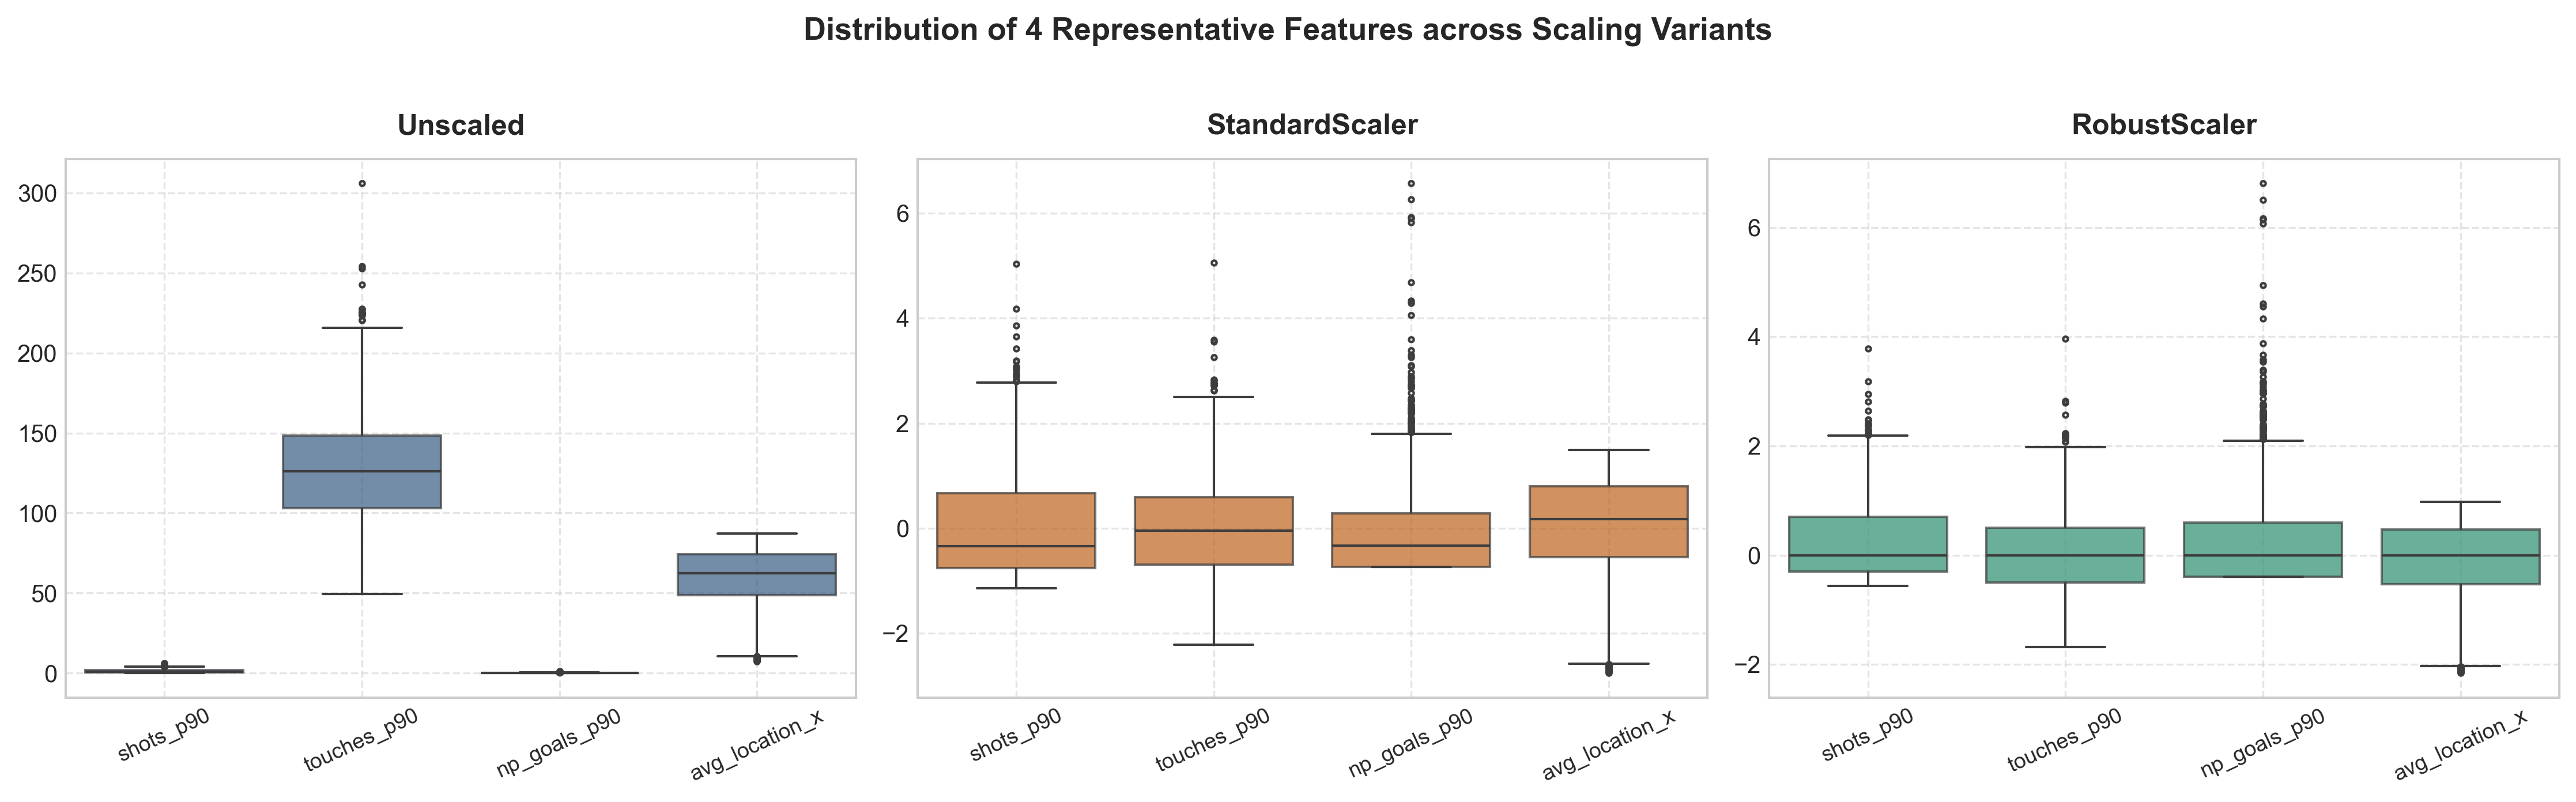
\includegraphics[width=0.85\linewidth]{figures/fig_scaling_boxplots.png}
    \begin{minipage}{0.85\linewidth}
    \begin{figurecaptionmodern}
        \raggedright
        \capfig{Distribution box plots across four representative features comparing Unscaled, StandardScaler, and RobustScaler data matrices.}
        \label{fig:scaling_boxplots}
    \end{figurecaptionmodern}
    \end{minipage}
\end{center}

In the unscaled data, \texttt{touches\_p90} ranges from $49.3$ to $305.9$ ($\sigma \approx 35.3$), whereas \texttt{np\_goals\_p90} only ranges from $0.0$ to $1.07$ ($\sigma \approx 0.147$). Because Euclidean distance squares difference values, a small difference in touch volume between two midfielders would outweigh a substantial difference in goal scoring between a striker and a defender.

To assess how scaling affects the resulting clusters, we measured pairwise Adjusted Rand Index (ARI) agreement across the three transformations at $k=5$ (Table~\ref{tab:ari_comparison}).

\begin{table}[H]
\centering
\begin{minipage}{0.8\linewidth}
  \refstepcounter{table}
  \begin{captionbelowboxaivn}
    Table~\thetable: Pairwise Adjusted Rand Index (ARI) agreement between scaling variants ($k=5$)
    \label{tab:ari_comparison}
  \end{captionbelowboxaivn}
  \renewcommand{\arraystretch}{1.3}
  \begin{tabularx}{\linewidth}{@{}>{\raggedright\arraybackslash}X >{\centering\arraybackslash}X@{}}
    \toprule
    \textbf{Scaling Strategy Pair} & \textbf{Adjusted Rand Index (ARI)} \\
    \midrule
    StandardScaler vs. RobustScaler & \textbf{0.971} \\
    Unscaled vs. StandardScaler & 0.342 \\
    Unscaled vs. RobustScaler & 0.355 \\
    \bottomrule
  \end{tabularx}
\end{minipage}
\end{table}

The high agreement between StandardScaler and RobustScaler ($\text{ARI} = 0.971$) indicates that both scaling methods produce consistent cluster structures. In contrast, the poor agreement with Unscaled clustering ($\text{ARI} \approx 0.35$) confirms that unscaled clustering is heavily distorted by touch volume. RobustScaler was chosen for all subsequent modeling because of its resilience to skewed distributions and outliers.

\subsection{Model Selection (RQ2)}
Figure~\ref{fig:k_selection} shows the model selection curves for $k \in [2, 10]$ on the RobustScaler feature space.

\begin{center}
    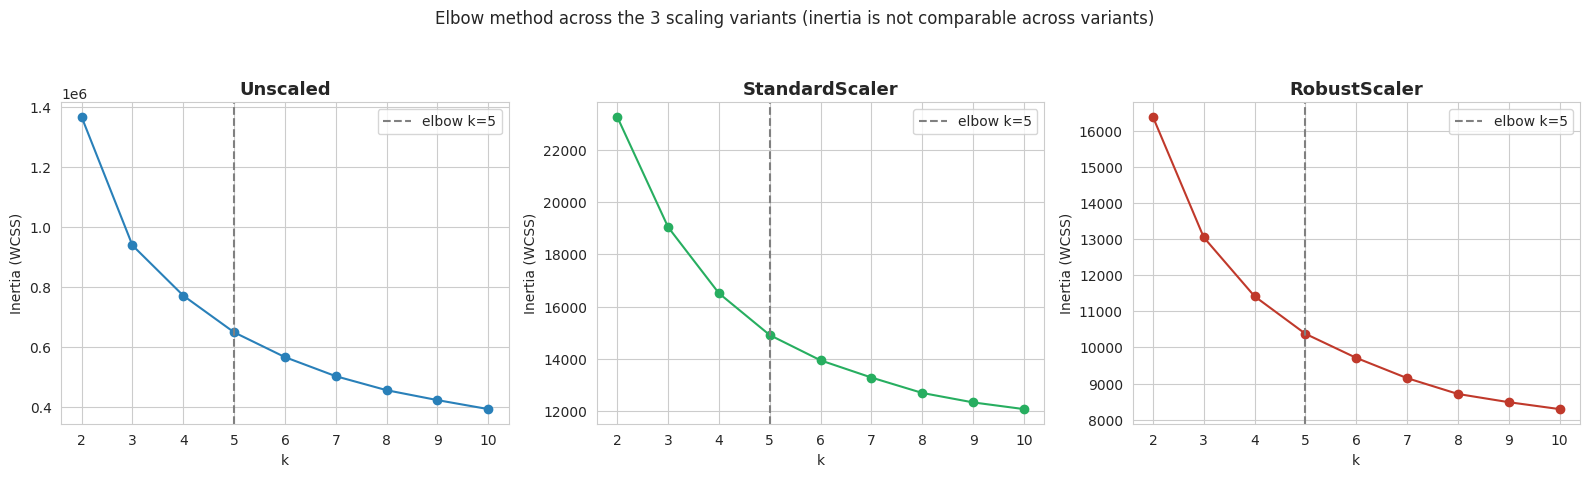
\includegraphics[width=0.95\linewidth]{figures/fig_k_elbow.png}\\[1ex]
    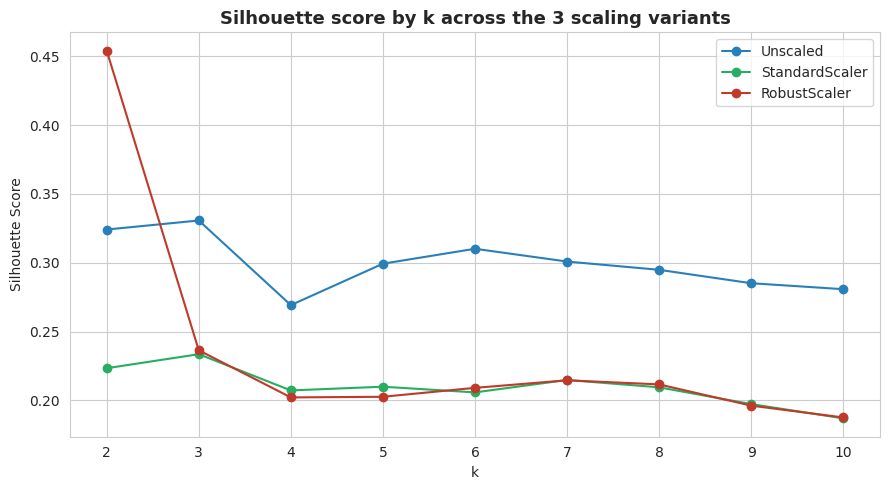
\includegraphics[width=0.95\linewidth]{figures/fig_k_silhouette.png}\\[1ex]
    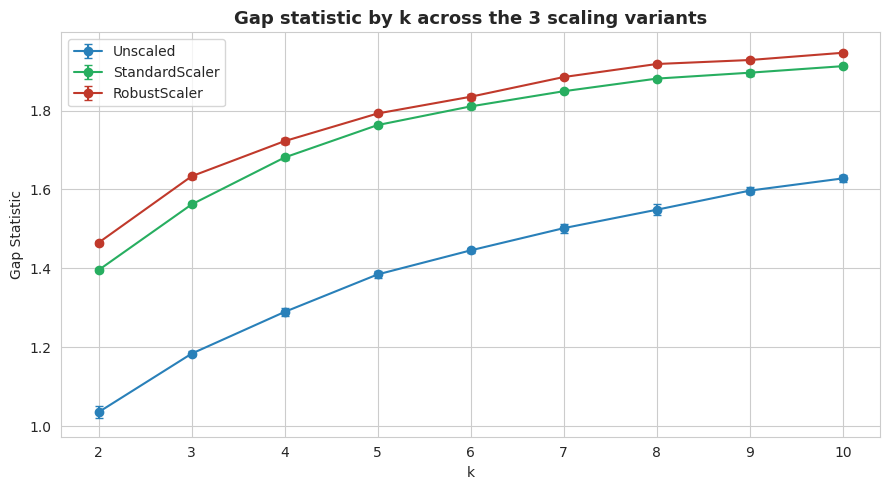
\includegraphics[width=0.95\linewidth]{figures/fig_k_gap.png}
    \begin{minipage}{0.95\linewidth}
    \begin{figurecaptionmodern}
        \raggedright
        \capfig{Model selection curves across scaling variants: (Top) Elbow WCSS curves, (Middle) Silhouette Scores, and (Bottom) Gap Statistic across $k \in [2, 10]$.}
        \label{fig:k_selection}
    \end{figurecaptionmodern}
    \end{minipage}
\end{center}

Analyzing the model selection curves provides key insights:
\begin{itemize}
  \item \textbf{Elbow Method (WCSS):} The WCSS curve drops steeply before flattening out around $k=5$, indicating diminishing returns from adding more clusters.
  \item \textbf{Silhouette Score:} The Silhouette score reaches its highest value at $k=2$ ($\approx 0.38$). However, inspecting $k=2$ shows that it merely creates a simple split between defensive and attacking players, which is too general for tactical analysis. At $k=5$, the Silhouette curve forms a clear local peak ($\approx 0.22$), providing a good separation between distinct tactical roles.
  \item \textbf{Gap Statistic:} The Gap Statistic increases steadily relative to the uniform reference distribution, supporting $k=5$ as a strong choice.
\end{itemize}

Based on both statistical metrics and practical interpretability, \textbf{$k=5$ is selected as the optimal number of clusters}.

\subsection{Positional Validation (RQ3)}
To evaluate whether the unsupervised clusters reflect meaningful football roles, the five K-Means clusters ($k=5$, RobustScaler) were cross-tabulated against the four broad ground-truth positions (Attack, Defense, Goalkeeper, Midfield), as shown in Table~\ref{tab:crosstab}.

\begin{table}[H]
\centering
\begin{minipage}{0.85\linewidth}
  \refstepcounter{table}
  \begin{captionbelowboxaivn}
    Table~\thetable: Contingency matrix comparing K-Means cluster assignments ($k=5$, RobustScaler) against actual positional groups
    \label{tab:crosstab}
  \end{captionbelowboxaivn}
  \renewcommand{\arraystretch}{1.3}
  \begin{tabularx}{\linewidth}{@{}>{\centering\arraybackslash}p{2cm}
      >{\centering\arraybackslash}X >{\centering\arraybackslash}X
      >{\centering\arraybackslash}X >{\centering\arraybackslash}X >{\centering\arraybackslash}X@{}}
    \toprule
    \textbf{Cluster ID} & \textbf{Attack} & \textbf{Defense} & \textbf{Goalkeeper} & \textbf{Midfield} & \textbf{Total Size} \\
    \midrule
    Cluster 0 & 0 & \textbf{189} & 0 & 5 & 194 \\
    Cluster 1 & \textbf{145} & 0 & 0 & 7 & 152 \\
    Cluster 2 & 0 & 0 & \textbf{73} & 0 & 73 \\
    Cluster 3 & 92 & 5 & 0 & \textbf{101} & 198 \\
    Cluster 4 & 10 & 189 & 0 & \textbf{200} & 399 \\
    \midrule
    \textbf{Total} & 247 & 383 & 73 & 313 & \textbf{1,016} \\
    \bottomrule
  \end{tabularx}
\end{minipage}
\end{table}

\begin{center}
    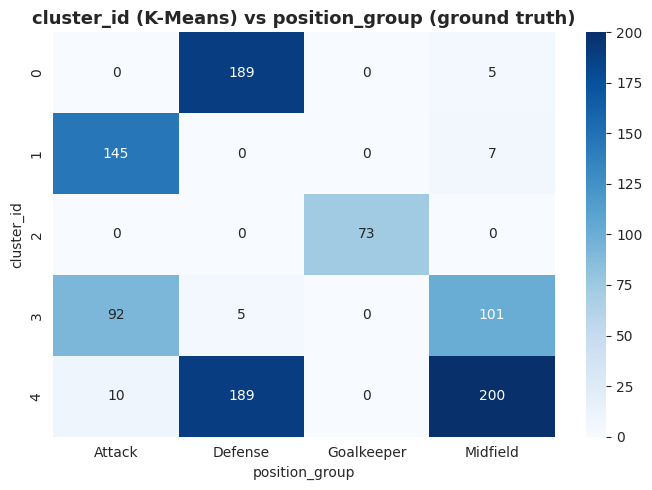
\includegraphics[width=0.75\linewidth]{figures/fig_cluster_position_heatmap.png}
    \begin{minipage}{0.75\linewidth}
    \begin{figurecaptionmodern}
        \raggedright
        \capfig{Heatmap matrix showing the alignment between K-Means clusters and actual position groups.}
        \label{fig:cluster_heatmap}
    \end{figurecaptionmodern}
    \end{minipage}
\end{center}

Quantitative evaluation of Table~\ref{tab:crosstab} shows strong correspondence with real positions:
\[
\text{Overall Purity} = \frac{189 + 145 + 73 + 101 + 200}{1016} = \frac{708}{1016} \approx 0.697 \quad (69.7\%)
\]
\[
\text{Normalized Mutual Information (NMI)} \approx 0.546
\]

Examining the feature values of each cluster reveals five clear tactical archetypes:
\begin{itemize}
  \item \textbf{Cluster 0 (Defensive Anchors \& Center-Backs -- 194 players):} Dominated by central defenders ($97.4\%$). Defined by high clearance rates (\texttt{clearances\_p90} $\approx 4.8$), aerial dominance, and deep pitch positioning (\texttt{avg\_location\_x} $\approx 41.3$).
  \item \textbf{Cluster 1 (Clinical Finishers \& Primary Forwards -- 152 players):} Mostly strikers ($95.4\%$). Characterized by high shot volume (\texttt{shots\_p90} $\ge 2.8$), non-penalty goals, and frequent touches in the box (\texttt{touches\_in\_box\_p90} $\ge 12.5$).
  \item \textbf{Cluster 2 (Goalkeepers -- 73 players):} Achieves $100\%$ pure separation ($73/73$). Defined by near-zero outfield actions and minimal progression upfield (\texttt{avg\_location\_x} $\approx 9.6$).
  \item \textbf{Cluster 3 (Creative Playmakers \& Dynamic Wingers -- 198 players):} Combines attacking midfielders ($51.0\%$) and wingers ($46.5\%$). Characterized by high key passes (\texttt{key\_passes\_p90} $\approx 1.8$), assists, crosses, and successful dribbles.
  \item \textbf{Cluster 4 (Possession Controllers \& Hybrid Fullbacks -- 399 players):} Blends central midfielders ($50.1\%$) and fullbacks ($47.4\%$). This reflects modern tactical systems, where fullbacks and central midfielders share high passing volumes, pressing actions, and ball recoveries.
\end{itemize}

\subsection{Cluster Stability and Learnability}
To test whether the cluster partitions form learnable boundaries in feature space, a K-Nearest Neighbors (KNN) classifier was trained to predict cluster labels under 5-fold Stratified Cross-Validation across neighbor values $n\_neighbors \in [5, 20]$ (Table~\ref{tab:knn_sweep}).

\begin{table}[H]
\centering
\begin{minipage}{0.8\linewidth}
  \refstepcounter{table}
  \begin{captionbelowboxaivn}
    Table~\thetable: KNN 5-fold cross-validation accuracy across varying neighbor parameter $n\_neighbors$
    \label{tab:knn_sweep}
  \end{captionbelowboxaivn}
  \renewcommand{\arraystretch}{1.3}
  \begin{tabularx}{\linewidth}{@{}>{\centering\arraybackslash}X >{\centering\arraybackslash}X >{\centering\arraybackslash}X@{}}
    \toprule
    \textbf{KNN Parameter ($n\_neighbors$)} & \textbf{Mean CV Accuracy} & \textbf{Standard Deviation} \\
    \midrule
    $k = 5$ & 0.954 & $\pm 0.011$ \\
    $k = 10$ & 0.961 & $\pm 0.009$ \\
    \textbf{$k = 15$ (Final Model)} & \textbf{0.966} & \textbf{$\pm 0.008$} \\
    $k = 20$ & 0.962 & $\pm 0.009$ \\
    \bottomrule
  \end{tabularx}
\end{minipage}
\end{table}

At $n\_neighbors=15$, the KNN model achieves a cross-validation accuracy of \textbf{$96.6\% \pm 0.8\%$}. This result confirms that the K-Means clusters form distinct and stable decision boundaries in the 29-dimensional space.

\begin{center}
    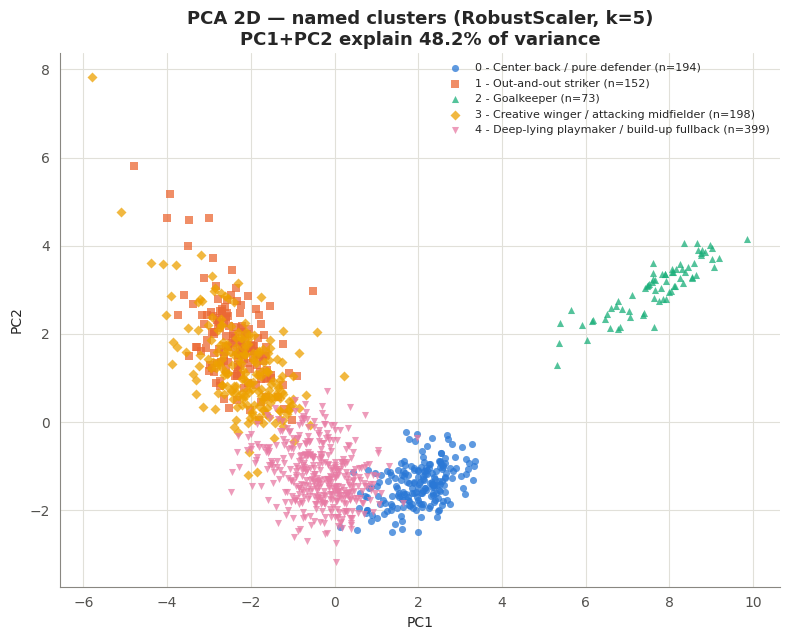
\includegraphics[width=0.85\linewidth]{figures/fig_pca_clusters.png}
    \begin{minipage}{0.85\linewidth}
    \begin{figurecaptionmodern}
        \raggedright
        \capfig{2D Principal Component Analysis (PCA) projection showing cluster separation across the first two principal components.}
        \label{fig:pca}
    \end{figurecaptionmodern}
    \end{minipage}
\end{center}

\begin{center}
    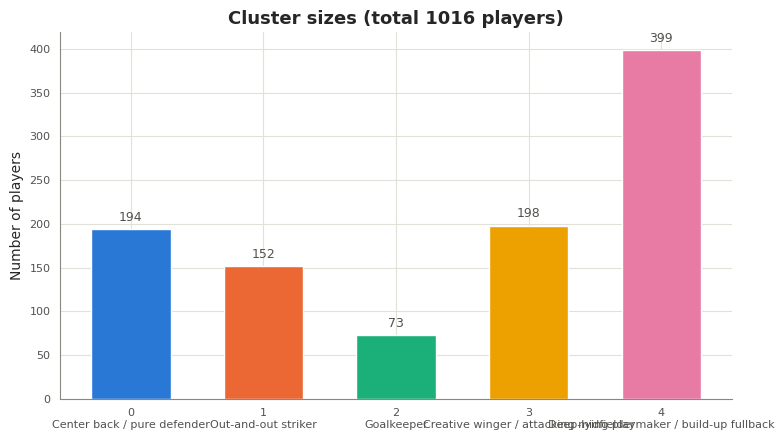
\includegraphics[width=0.85\linewidth]{figures/fig_radar_clusters.png}
    \begin{minipage}{0.85\linewidth}
    \begin{figurecaptionmodern}
        \raggedright
        \capfig{Radar chart mapping cluster centroid feature profiles across attacking, creative, defensive, and spatial dimensions.}
        \label{fig:radar}
    \end{figurecaptionmodern}
    \end{minipage}
\end{center}

Figure~\ref{fig:pca} shows the 2D Principal Component Analysis (PCA) projection, confirming visible cluster separation. Figure~\ref{fig:radar} illustrates the centroid radar profiles, highlighting the distinct behavioral differences across attacking, creative, defensive, and spatial metrics.

\subsection{Case Study: Fine-Grained Tactical Sub-Clustering of Primary Forwards}
\label{sec:striker_subclustering}

The five macro-clusters provide a broad view of player roles across the pitch. As a case study, we apply a secondary K-Means clustering step specifically on \textbf{Cluster 1 (Clinical Finishers \& Primary Forwards, $n = 152$)} to show that the pipeline can be extended hierarchically to discover more specific tactical roles within a single position.

\subsubsection{Feature Selection for the Striker Subspace}

Within this 152-player group, 12 features from the full 29-feature matrix are near-constant or uninformative (such as \texttt{clearances\_p90}, \texttt{tackles\_p90}, and \texttt{interceptions\_p90}) and are removed. In contrast, an important feature not included in the macro pipeline is added: \texttt{passes\_p90}. This 17-feature matrix is then scaled using \texttt{RobustScaler} fitted only on the 152 strikers.

\textbf{Note on scoring metrics:} \texttt{np\_goals\_p90} and \texttt{assists\_p90} are kept in this subgroup because, among forwards in similar positions, they help distinguish box finishers from link-up forwards.

\subsubsection{Hyperparameter Evaluation ($k \in [2, 7]$)}

We test candidate values of $k \in [2, 7]$ on the scaled 17-feature striker data using the Elbow method, Silhouette Score, and Gap Statistic (Figure~\ref{fig:striker_k_selection}).

\begin{center}
    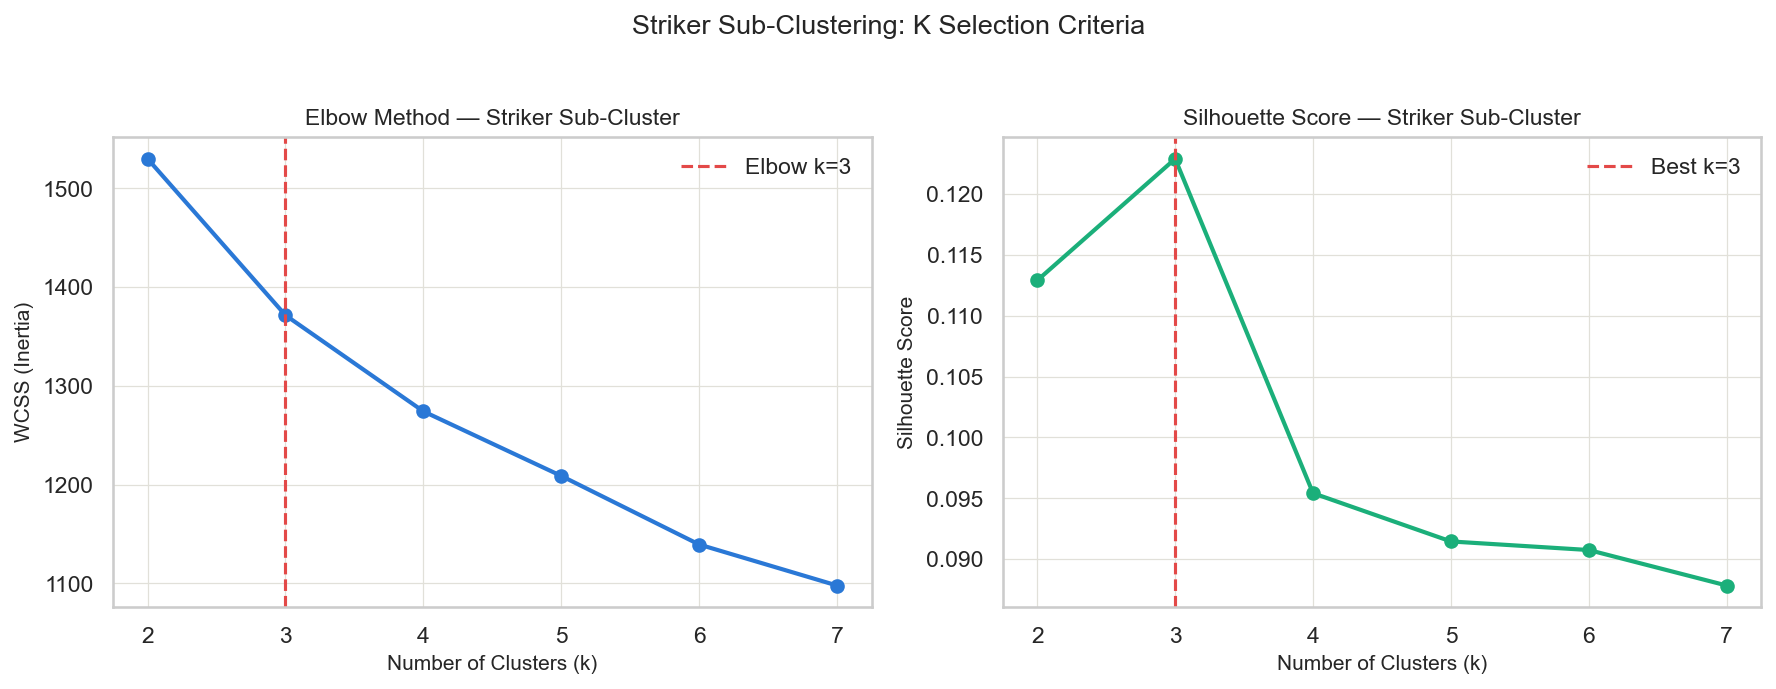
\includegraphics[width=0.90\linewidth]{figures/fig_striker_k_selection.png}
    \begin{minipage}{0.90\linewidth}
    \begin{figurecaptionmodern}
        \raggedright
        \capfig{Striker sub-cluster hyperparameter evaluation: Elbow curve (WCSS, left) and Silhouette score (right) over $k \in [2, 7]$.}
        \label{fig:striker_k_selection}
    \end{figurecaptionmodern}
    \end{minipage}
\end{center}

\subsubsection{Initial Candidate ($k = 4$): The Superstar Outlier Effect}

Although the Gap Statistic and Silhouette curve suggest $k = 4$, closer inspection reveals a common issue in clustering: \emph{clustering on player quality rather than playing style}.

When $k = 4$ is fitted, the forwards are split into four clusters ($n = 57, 16, 23, 56$). In particular, \textbf{Cluster 1 ($n = 16$)} isolates a group of world-class forwards: Karim Benzema, Luis Su\'arez, Gonzalo Higu\'ain, Gareth Bale, Cristiano Ronaldo, Sergio Ag\"uero, Antoine Griezmann, Romelu Lukaku, Harry Kane, and Mohamed Salah.

\begin{center}
    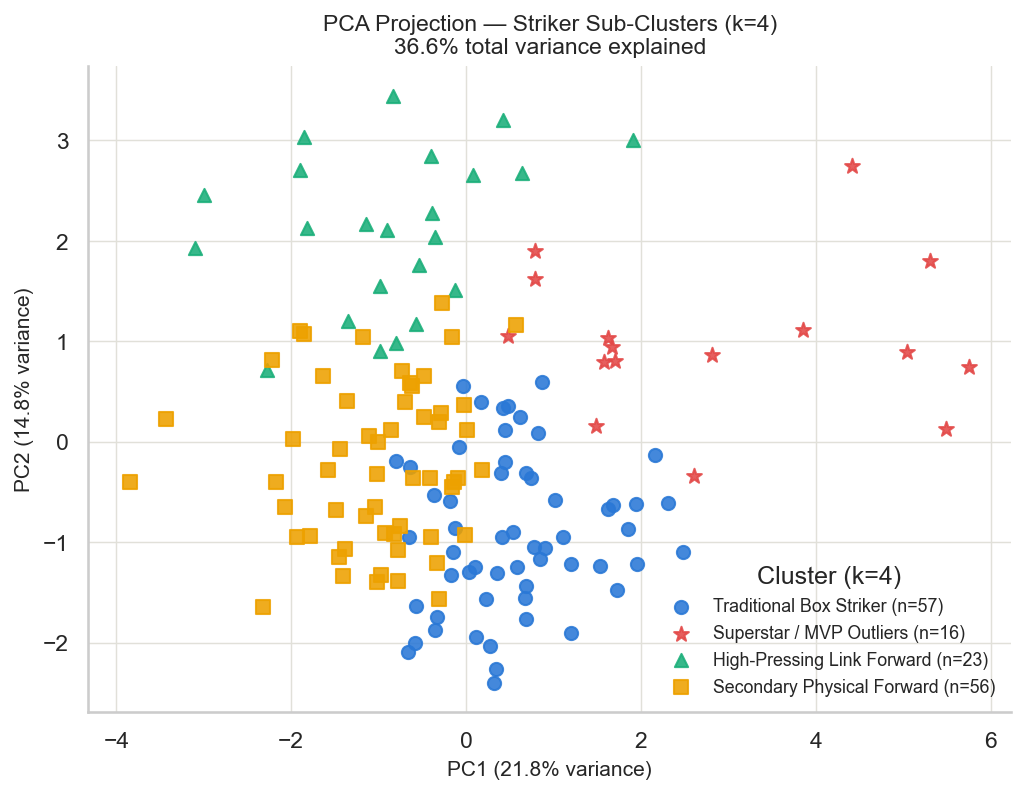
\includegraphics[width=0.82\linewidth]{figures/fig_striker_k4_pca.png}
    \begin{minipage}{0.82\linewidth}
    \begin{figurecaptionmodern}
        \raggedright
        \capfig{2D PCA projection of the 152 forwards under $k=4$, highlighting the outlier cluster of elite forwards (Cluster 1, red stars, $n=16$).}
        \label{fig:striker_k4_pca}
    \end{figurecaptionmodern}
    \end{minipage}
\end{center}

\begin{center}
    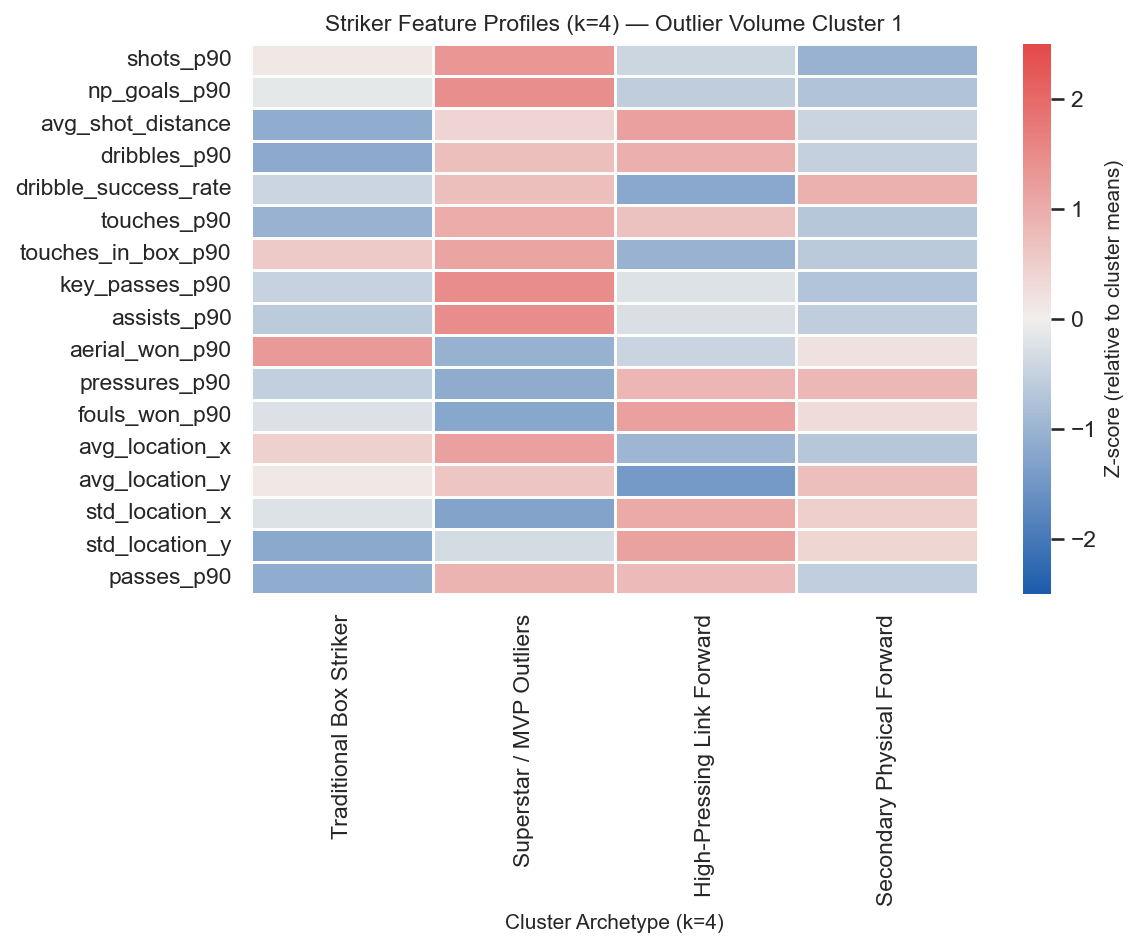
\includegraphics[width=0.85\linewidth]{figures/fig_striker_k4_profiles.png}
    \begin{minipage}{0.85\linewidth}
    \begin{figurecaptionmodern}
        \raggedright
        \capfig{Z-score centroid feature heatmap for $k = 4$. Cluster 1 shows high positive values across nearly all attacking metrics simultaneously, reflecting overall quality rather than a distinct tactical style.}
        \label{fig:striker_k4_profiles}
    \end{figurecaptionmodern}
    \end{minipage}
\end{center}

As shown in Figure~\ref{fig:striker_k4_profiles}, Cluster 1 players lead in almost every attacking category: they average $0.65$ non-penalty goals p90, $3.63$ shots p90, $18.38$ box touches p90, $30.83$ passes p90, and $1.22$ key passes p90. Because their output volume is high across the board, K-Means groups them based on \textbf{overall performance volume} rather than \textbf{functional tactical role}.

Moreover, separating this group splits the remaining 136 players awkwardly:
\begin{enumerate}
    \item \textbf{Target Man dilution:} Physical forwards are split between Cluster 0 ($n = 57$) and Cluster 3 ($n = 56$), reducing the aerial dominance ratio over other clusters from $1.73\times$ (under $k=3$) to $1.47\times$ (under $k=4$).
    \item \textbf{Poacher fragmentation:} Elite penalty-box finishers (such as Su\'arez, Ronaldo, and Ag\"uero) are separated from other box poachers into the superstar cluster, blurring the definition of the Poacher archetype.
\end{enumerate}

\subsubsection{Model Refinement ($k = 3$): Tactical Archetype Discovery}

To avoid this quality-based distortion and isolate true tactical styles, we set $k = 3$. Under $k = 3$, top forwards fit naturally into tactical archetypes according to their pitch positioning and playing style (e.g., Su\'arez and Ronaldo in the Poacher group; Benzema in Deep-Lying Forwards) rather than forming an isolated group.

Table~\ref{tab:striker_centroids} summarizes the centroid values for the three tactical archetypes under $k = 3$.

\begin{table}[H]
\centering
\begin{minipage}{1.0\linewidth}
  \refstepcounter{table}
  \begin{captionbelowboxaivn}
    Table~\thetable: Mean (unscaled) centroid feature values for the three refined striker tactical archetypes ($k = 3$, $n = 152$)
    \label{tab:striker_centroids}
  \end{captionbelowboxaivn}
  \renewcommand{\arraystretch}{1.3}
  \begin{tabularx}{\linewidth}{@{}>{\raggedright\arraybackslash}p{4.2cm}
      >{\centering\arraybackslash}X >{\centering\arraybackslash}X >{\centering\arraybackslash}X@{}}
    \toprule
    \textbf{Feature} &
    \textbf{Cluster 0} & \textbf{Cluster 1} & \textbf{Cluster 2} \\
    & \textbf{Deep-Lying Fwd.} & \textbf{Target Man} & \textbf{Poacher} \\
    & ($n = 52$) & ($n = 82$) & ($n = 18$) \\
    \midrule
    \texttt{touches\_in\_box\_p90}  & 11.41        & 13.97        & \textbf{23.36} \\
    \texttt{shots\_p90}            & 2.16         & 2.21         & \textbf{4.26}  \\
    \texttt{np\_goals\_p90}        & 0.26         & 0.28         & \textbf{0.75}  \\
    \texttt{aerial\_won\_p90}      & 1.95         & \textbf{3.86}& 1.70           \\
    \texttt{passes\_p90}          & \textbf{30.81}& 21.75       & 29.83          \\
    \texttt{avg\_location\_x}     & 77.41        & 79.52        & \textbf{82.37} \\
    \texttt{pressures\_p90}       & \textbf{17.58}& 14.86       & 11.83          \\
    \bottomrule
  \end{tabularx}
\end{minipage}
\end{table}

\begin{itemize}
  \item \textbf{Poacher / Clinical Box Finisher (Cluster 2, $n = 18$):} Characterized by high penalty-box presence ($\texttt{touches\_in\_box\_p90} = 23.36$), high shot volume ($4.26$ p90), high non-penalty goals ($0.75$ p90), and advanced pitch positioning ($\texttt{avg\_location\_x} = 82.37$), with lower defensive work ($11.83$ pressures p90). Examples include Luis Su\'arez, Cristiano Ronaldo, Gonzalo Higu\'ain, Sergio Ag\"uero, and Daniel Sturridge.
  \item \textbf{Target Man / Aerial Reference Point (Cluster 1, $n = 82$):} Physical forwards defined by aerial strength ($\texttt{aerial\_won\_p90} = 3.86$, nearly double the deep-lying forwards) and hold-up play, along with the lowest passing volume in the forward group ($\texttt{passes\_p90} = 21.75$). Examples include Salom\'on Rond\'on, Mario Mand\v{z}uki\'c, Romelu Lukaku, Christian Benteke, and Graziano Pell\`e.
  \item \textbf{Deep-Lying Forward (Cluster 0, $n = 52$):} Forwards who drop deeper into midfield ($\texttt{avg\_location\_x} = 77.41$), recording the highest passing volume ($\texttt{passes\_p90} = 30.81$) and most defensive pressing ($\texttt{pressures\_p90} = 17.58$). Examples include Son Heung-Min, Theo Walcott, Nacer Chadli, and Borja Bast\'on.
\end{itemize}

Figures~\ref{fig:striker_pca}, \ref{fig:striker_profiles}, and~\ref{fig:striker_pitch} illustrate the clear spatial and behavioral differences between the three archetypes under $k = 3$.

\begin{center}
    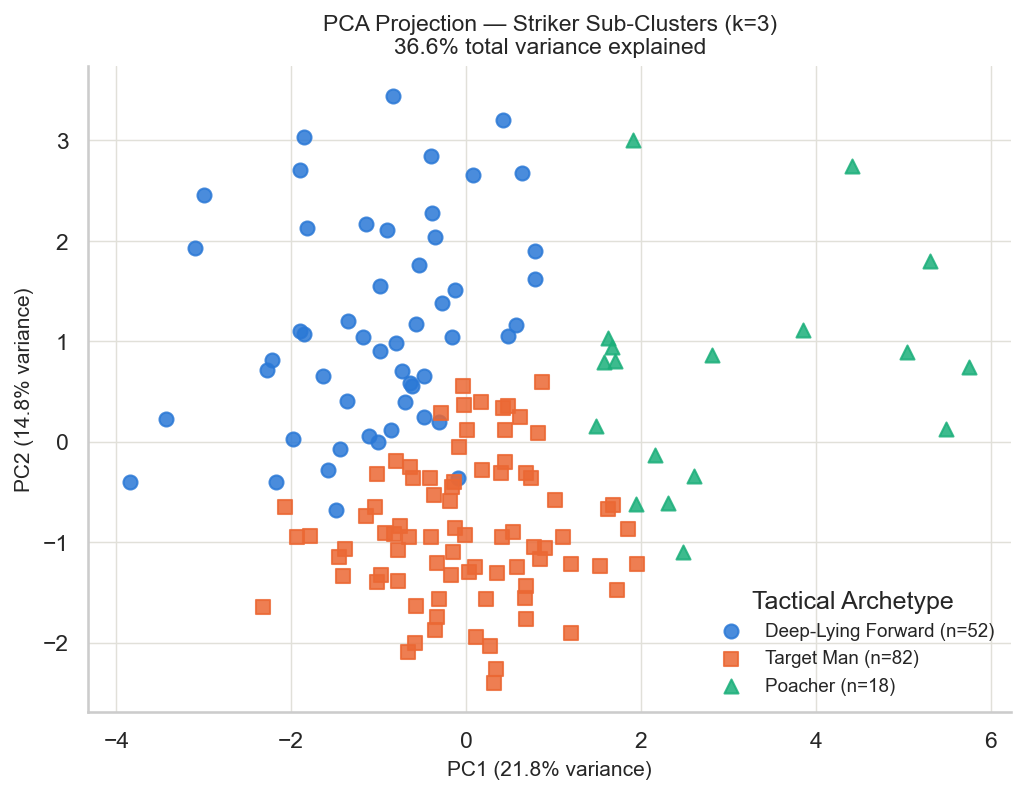
\includegraphics[width=0.80\linewidth]{figures/fig_striker_pca.png}
    \begin{minipage}{0.80\linewidth}
    \begin{figurecaptionmodern}
        \raggedright
        \capfig{2D PCA projection of the 152 forwards under $k = 3$, showing clear separation between Deep-Lying Forwards, Target Men, and Poachers.}
        \label{fig:striker_pca}
    \end{figurecaptionmodern}
    \end{minipage}
\end{center}

\begin{center}
    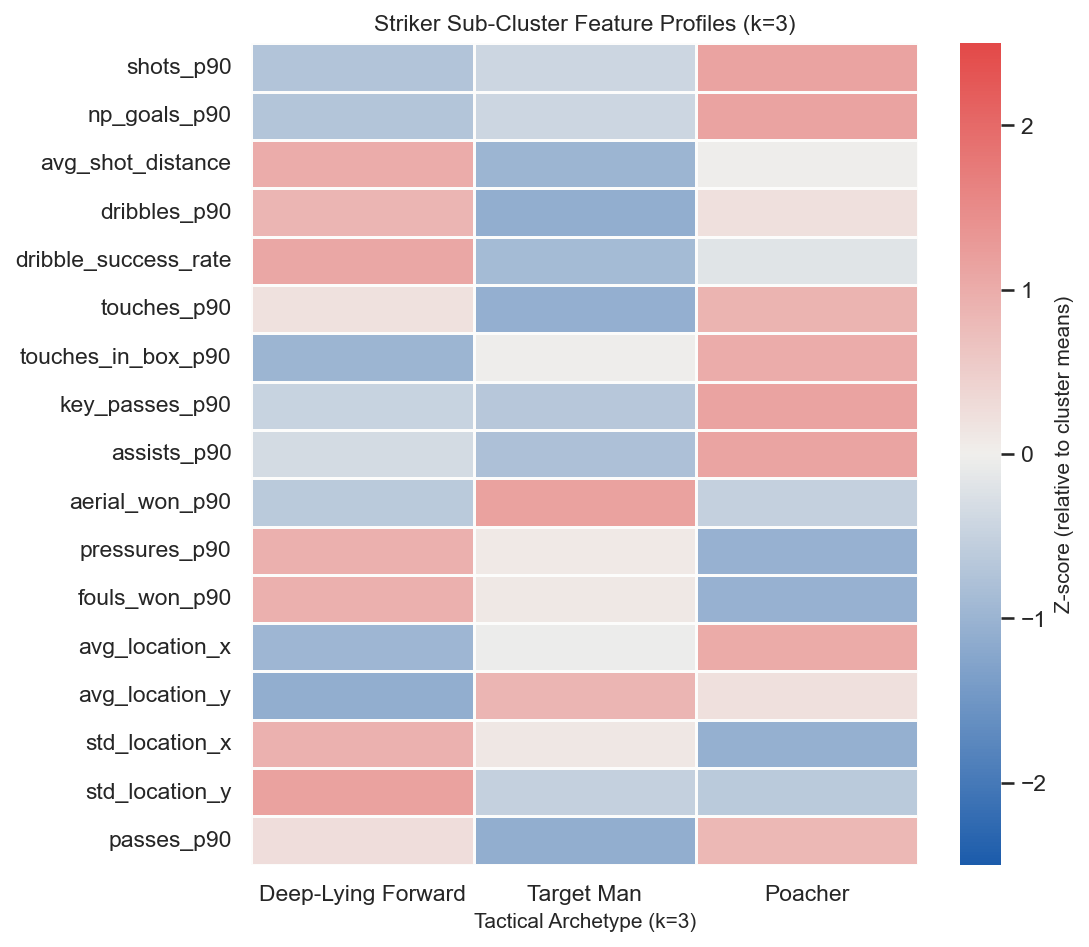
\includegraphics[width=0.80\linewidth]{figures/fig_striker_profiles.png}
    \begin{minipage}{0.80\linewidth}
    \begin{figurecaptionmodern}
        \raggedright
        \capfig{Centroid feature heatmap (Z-score normalized across sub-clusters) for the three striker archetypes ($k = 3$), confirming distinct profiles across box finishing, aerial duels, and link-up play.}
        \label{fig:striker_profiles}
    \end{figurecaptionmodern}
    \end{minipage}
\end{center}

\begin{center}
    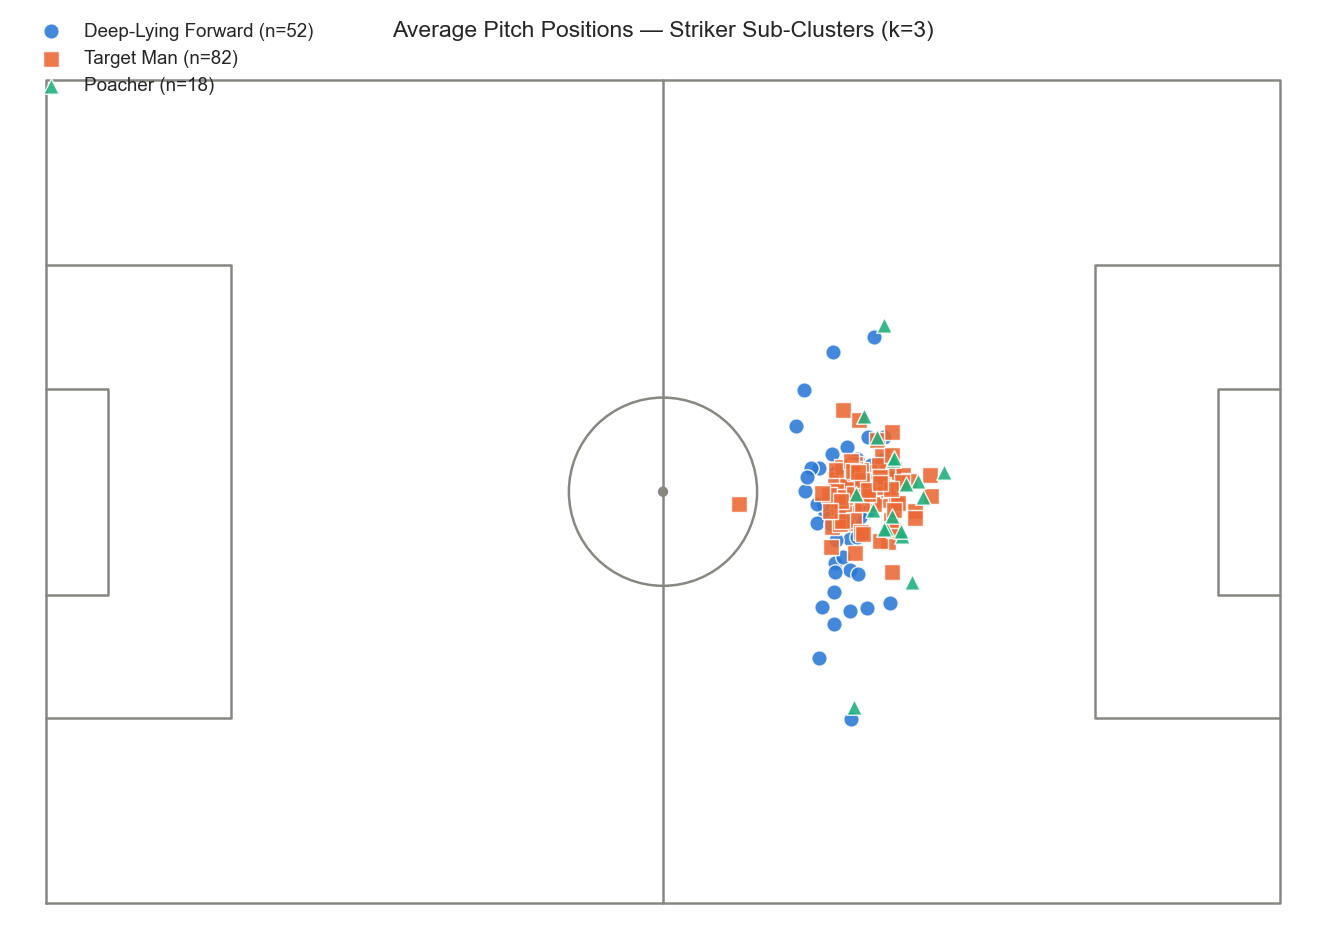
\includegraphics[width=0.80\linewidth]{figures/fig_striker_pitch.png}
    \begin{minipage}{0.80\linewidth}
    \begin{figurecaptionmodern}
        \raggedright
        \capfig{Average seasonal pitch locations of the 152 forwards ($k = 3$). The longitudinal coordinate clearly separates Deep-Lying Forwards ($x \approx 77.4$) from Target Men ($x \approx 79.5$) and Poachers ($x \approx 82.4$).}
        \label{fig:striker_pitch}
    \end{figurecaptionmodern}
    \end{minipage}
\end{center}

\subsubsection{Methodological Takeaway}

The comparison between $k = 4$ and $k = 3$ highlights an important lesson in sports clustering: \textbf{clustering algorithms can easily group players by overall quality rather than playing style when performance volume varies widely}. By adjusting features for the specific subspace (\texttt{passes\_p90}) and selecting $k = 3$, we obtain a clear, practical classification of forward roles.

% --------------------------------------------------------------------------
\section{Discussion and Applications}
\label{sec:discussion}

The findings from this study offer practical applications for football analytics and scouting:

\subsection{Player Scouting and Recruitment}
Traditional scouting can face difficulties when trying to replace players with unique tactical roles. For example, if a team loses an attacking fullback who functions as an inverted creator, searching only for "Right Backs" on team sheets may overlook suitable candidates playing in midfield. By mapping players into the 29-dimensional feature space, clubs can compute Euclidean distances to a target centroid to find players with matching playing styles regardless of their nominal position.

\subsection{Opposition Tactical Analysis}
By looking at the cluster assignments of an opponent's starting lineup across recent matches, coaching staffs can construct an objective tactical overview of the team. For instance, knowing whether an opponent uses two traditional wingers (Cluster 3) or two central creators (Cluster 4) can help teams prepare their defensive structure and pressing tactics accordingly.

\subsection{Limitations and Future Work}
While the results show good stability and interpretability, some limitations should be noted:
\begin{enumerate}
  \item \textbf{Seasonal Aggregation:} Season-level averages provide statistical stability but overlook match-to-match changes in tactics, player fitness, or role shifts under different managers.
  \item \textbf{Equal Weighting of Events:} Standard per-90 rates treat all actions equally, without accounting for match state (e.g., leading vs. trailing) or the quality of opposition.
\end{enumerate}
Future work could include possession-value metrics (such as Expected Threat / xT), tracking data for off-ball movement, and multi-season tracking to observe how player roles evolve over time.

% --------------------------------------------------------------------------
\section{Conclusion}
\label{sec:conclusion}

This study presents a structured analysis of unsupervised player style clustering using football event data. By addressing feature scaling, cluster selection, and stability validation on 1,016 players from the 2015/2016 season, our main conclusions are:
\begin{enumerate}
  \item \textbf{Feature scaling is critical:} RobustScaler normalization based on medians and interquartile ranges is necessary to prevent extreme performance values from dominating distance-based clustering.
  \item \textbf{Five tactical archetypes:} Model selection metrics and tactical interpretability identify $k=5$ as the most suitable choice, grouping players into Center-Backs, Strikers, Goalkeepers, Playmakers/Wingers, and Possession Controllers.
  \item \textbf{High cluster stability:} The clusters correspond well to actual positions ($\text{Purity} \approx 69.7\%$) and show stable boundaries confirmed by a $96.6\%$ KNN cross-validation accuracy.
  \item \textbf{Extensibility to sub-clustering:} A secondary clustering step on the 152 strikers identifies three distinct styles (Poachers, Target Men, and Deep-Lying Forwards), demonstrating that the framework can be applied hierarchically for more detailed role discovery.
\end{enumerate}

This framework provides an effective, data-driven foundation for player profiling and tactical analysis in modern football.

% --------------------------------------------------------------------------
\newpage
\printbibliography

% --------------------------------------------------------------------------
\newpage
\begin{appendices}

\begin{enumerate}
  \item \textbf{AIVIETNAM Program:} Details regarding AI VIETNAM curriculum, coursework, and initiatives are accessible at \href{https://aivietnam.edu.vn/}{aivietnam.edu.vn}.
  \item \textbf{GitHub Repository:} Project implementation source code, exploratory notebooks, and pipeline scripts are available at \url{https://github.com/AIVIETNAM-AIO-Kaisye/player-style-clustering}.
  \item \textbf{Data Sources:} Open event data provided by StatsBomb (\url{https://github.com/statsbomb/open-data}) and mirror dataset on Kaggle (\url{https://www.kaggle.com/datasets/saurabhshahane/statsbomb-football-data}).
  \item \textbf{Execution Environment:} Experiments were conducted in Python 3.12 using \texttt{scikit-learn}, \texttt{pandas}, \texttt{numpy}, \texttt{matplotlib}, and \texttt{seaborn}.
  \item \textbf{Notebook Suite:}
  \begin{itemize}
    \item \texttt{01\_data\_and\_eda.ipynb}: Data ingestion, feature extraction, and EDA.
    \item \texttt{02\_modeling.ipynb}: Preprocessing, scaling comparison, and K-Means modeling.
    \item \texttt{03\_evaluation.ipynb}: Cluster validation (purity, NMI) and KNN stability.
    \item \texttt{04\_master\_pipeline.ipynb}: End-to-end combined pipeline.
    \item \texttt{05\_striker\_subclustering.ipynb}: Striker tactical sub-clustering case study.
  \end{itemize}
  \item \textbf{Author Contributions:}
  \begin{itemize}
    \item \textbf{Nguyễn Thanh Phong (Team Lead):} Repository infrastructure, master pipeline orchestration, and technical code review.
    \item \textbf{Võ Công Tuấn Lộc (Data Engineer):} Event aggregation logic, minute extraction algorithms, and exploratory data analysis.
    \item \textbf{Trương Hoàng Thông (ML \& Eval Engineer):} Preprocessing transformations, K-Means modeling, validation metrics, stability testing, and report formulation.
  \end{itemize}
\end{enumerate}

\end{appendices}

\end{document}
